\documentclass[a4paper,oneside]{article}

\usepackage[utf8]{inputenc}
\usepackage[brazil]{babel}
\usepackage{bookman}
\usepackage{ulem}
\usepackage{amssymb}
\usepackage{amsthm}
\usepackage{amsmath}
\usepackage{mathrsfs}
\usepackage{xspace}
\usepackage{enumerate}
\usepackage{makeidx}
\usepackage{calc}
\usepackage{ifthen}
\usepackage{epsfig}
\usepackage[portugues,vlined,boxruled,linesnumbered]{algorithm2e}

\setlength{\headheight}{0mm}
\setlength{\headsep}{0mm}
\setlength{\textheight}%
  {\paperheight-\footskip-\headsep-\headheight-\topmargin-\voffset-2in}
\setlength{\marginparwidth}{0mm}
\setlength{\marginparsep}{0mm}
\setlength{\textwidth}%
  {\paperwidth-\marginparwidth-\marginparsep-\oddsidemargin-\hoffset-2in}

\def\MMe{\mathrm{e}}
\def\MMi{\mathrm{i}}
\def\MMd{\mathrm{d}}
\def\MMN{\mathbb{N}}
\def\MMZ{\mathbb{Z}}
\def\MMQ{\mathbb{Q}}
\def\MMQbar{\overline{\mathbb{Q}}}
\def\MMR{\mathbb{R}}
\def\MMC{\mathbb{C}}
\def\MMP{\mathbb{P}}
\def\MME{\mathbb{E}}
\def\MMp{\mathrm{.}}
\def\MMv{\mathrm{,}}
\def\MMpv{\mathrm{;}}
\def\Hdie{\mathscr{H}}
\def\Rdie{\mathscr{R}}
\def\Var{\mathrm{Var}}
\def\geq{\geqslant}
\def\leq{\leqslant}
\def\divd{\backslash}
\def\ndivd{\not{\backslash}}
\def\parenteses#1{\left(#1\right)}
\def\colchetes#1{\left[\,#1\,\right]}
\def\colc#1{\colchetes{#1}}
\def\chaves#1{\left\{#1\right\}}
\def\cardi#1{\left|\,#1\,\right|}
\def\chao#1{\left\lfloor #1\right\rfloor}
\def\teto#1{\left\lceil #1\right\rceil}
\def\funcao#1#2#3{#1\colon #2\rightarrow #3}
\def\funcaom#1#2#3{#1\colon #2\mapsto #3}
\def\cj#1{\chaves{#1}}
\def\cjbar#1#2{\chaves{#1\text{ }\left|\text{ }#2\right.}}
\def\cjpp#1#2{\chaves{#1\colon#2}}
\def\galois#1{\mathbb{F}_{#1}}
\def\cquoc#1#2{{#1}_{{\displaystyle\diagup}_{\displaystyle{#2}}}}
\def\tcquoc#1#2{^{#1}{\scriptstyle\diagup}_{{#2}}}
\def\um{\underline{1}}
\def\zero{\underline{0}}
\def\congmod#1#2#3{#1\equiv #2\quad(\modu #3)}
\def\congmoda#1#2#3{#1&\equiv #2&\quad&(\modu #3)}
\def\gerado#1{\langle #1\rangle}
\def\potfatcresc#1#2{{#1}^{\overline{#2}}}
\def\potfatdecresc#1#2{{#1}^{\underline{#2}}}
\def\cleq#1#2{[#1]_{#2}}
\def\congmodright#1#2#3{#1\sim #2\quad(\modu #3)}
\def\congmodrighta#1#2#3{#1&\sim #2&\quad&(\modu #3)}
\def\congmodleft#1#2#3{#1\backsim #2\quad(\modu #3)}
\def\congmodlefta#1#2#3{#1&\backsim #2&\quad&(\modu #3)}
\def\id{\mathrm{id}}
\def\vetor#1{\boldsymbol{#1}}
\def\bfmais{\boldsymbol{+}}
\def\bfvezes{\boldsymbol{\cdot}}
\def\bfmenos{\boldsymbol{-}}
\def\bfzero{\boldsymbol{0}}
\def\nequiv{\not\equiv}
\def\SE{\Longrightarrow}
\def\wse{\text{\textsc{se }}}
\def\wentao{\text{\textsc{ ent\~ao }}}
\def\we{\text{\textsc{ e }}}
\def\recebe{\leftarrow}
\def\stirlingum#1#2{\genfrac{[}{]}{0pt}{}{#1}{#2}}
\def\stirlingdois#1#2{\genfrac{\{}{\}}{0pt}{}{#1}{#2}}
\def\tende{\rightarrow}
\def\crit#1{{#1}_{\mathrm{crit}}}
\def\ncrit#1{{#1}_{\mathrm{ncrit}}}

\makeatletter
  \def\sen{\mathop{\operator@font sen}\nolimits}
  \def\arcsen{\mathop{\operator@font arcsen}\nolimits}
  \def\diam{\mathop{\operator@font diam}}
  \def\cin{\mathop{\operator@font cin}}
  \def\dist{\mathop{\operator@font dist}}
  \def\ord{\mathop{\operator@font ord}}
  \def\mmc{\mathop{\operator@font mmc}}
  \def\mdc{\mathop{\operator@font mdc}}
  \def\gr{\mathop{\operator@font gr}}
  \def\dgr{\mathop{\operator@font d}}
  \def\modu{\mathop{\operator@font mod}}
\makeatother

\def\linmb#1{\textbf{\scriptsize #1}}
\def\upo{\textsuperscript{\d o}\xspace}
\def\hashing{\textit{hashing}\xspace}
\def\Hashing{\textit{Hashing}\xspace}
\def\hashings{\textit{hashings}\xspace}
\def\Hashings{\textit{Hashings}\xspace}

\newtheoremstyle{teoaxicorlem}%
  {}{}{\slshape}{}{\bfseries\scshape}{.}{ }{}
\newtheoremstyle{defnotnom}%
  {}{}{\upshape}{}{\bfseries\scshape}{.}{ }{}

\theoremstyle{defnotnom}
  \newtheorem{Def}{Definição}
  \newtheorem{Obs}[Def]{Observação}
  \newtheorem{Ex}[Def]{Exemplo}
\theoremstyle{teoaxicorlem}
  \newtheorem{Teo}[Def]{Teorema}
  \newtheorem{Cor}[Def]{Corolário}
  \newtheorem{Lem}[Def]{Lema}
  \newtheorem{Probl}[Def]{Problema}

\renewcommand{\qedsymbol}{$\blacklozenge$}

\newenvironment{prova}%
	{\begin{proof}[\scshape Prova.]}%
	{\end{proof}}
\newenvironment{dem}%
	{\begin{proof}[\scshape Demonstração.]}%
	{\end{proof}}

\graphicspath{{../Misc/Images/}}

\title{\Large\bfseries Rascunho de Notas de Estudo sobre\\
\Huge \Hashing Perfeita}
\author{\normalsize Leandro Zatesko\hspace{0.7in}
   {\footnotesize Orientador:} Prof. Dr. Jair Donadelli Jr.\\
   \texttt{\normalsize
     http://www.inf.ufpr.br/$\{$leandro$,$jair$\}$}%
   \\[0.1in]
   \protect\parbox[t]{2.2in}{%
     \noindent\centering%
     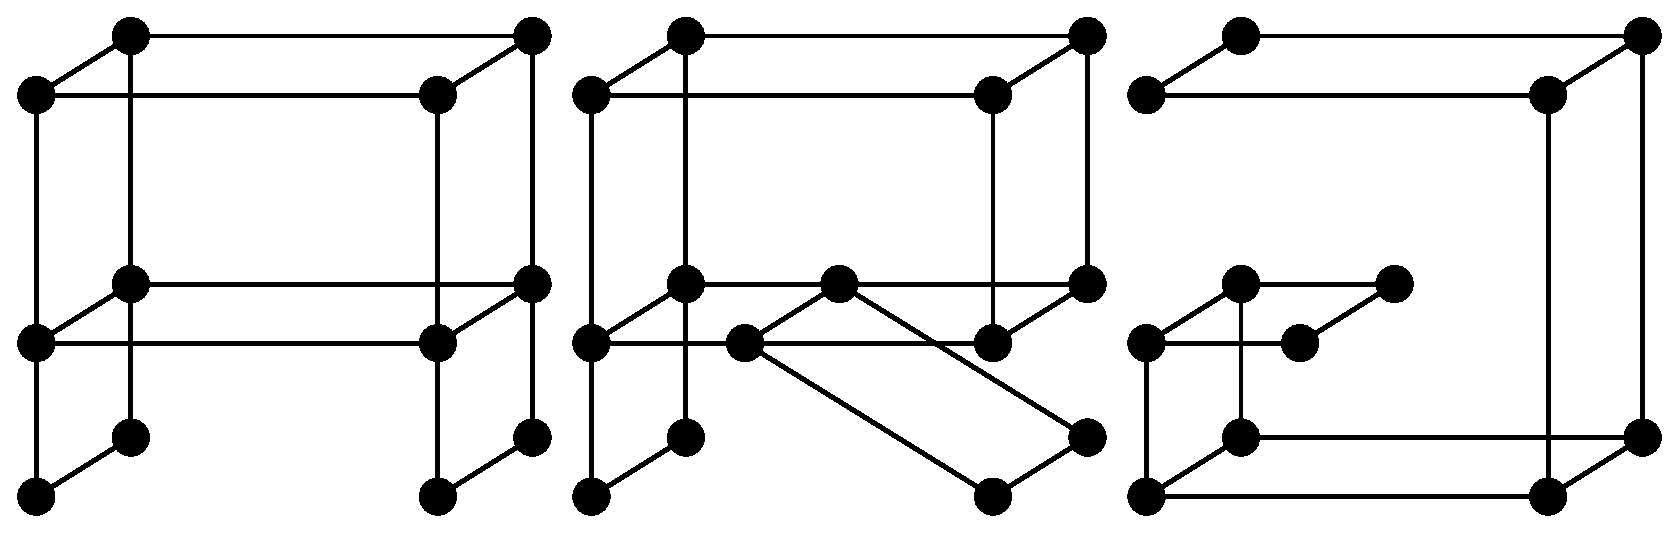
\epsfig{file=arg.eps,height=0.5in}\\%
     \normalsize\itshape Algorithms Research Group%
   }\hspace{0.7in}
   \protect\parbox[t]{2.2in}{%
     \noindent\centering%
     \epsfig{file=ufpr.eps,height=0.5in}\\%
     \normalsize Universidade Federal do Paraná%
   }\\[0.1in]
  \normalsize Mestrado em Ciência da Computação
}
\date{}

\renewcommand{\baselinestretch}{1.2}

\begin{document}

\maketitle

\tableofcontents

\section{Czech, Havas e Majewski}

Czech, Havas e Majewski propuseram um método de construção de hashing perfeita mínima que utiliza grafos aleatórios. O artigo de Botelho, Kohayakawa e Ziviani propõe um esquema fortemente baseado, com algumas modificações. No original, os grafos precisavam ser acíclicos, enquanto que agora eles precisam ser cíclicos. Tal como no original, entretanto, $|V|=cn$ e $|E|=|S|=n$. Mas, no original, $c=2.09$; agora $c=1.15$. Por outro lado, o esquema de representação de Botelho et al. não gera hashings que preservam a ordem nna tabela hash.

\section{Trabalhos relacionados}

\begin{description}
\item[Fredman, Komlós e Szemerédi] É possível construir funções hash perfeitas de tempo constante com tabelas cujos tamanhos são lineares no número das chaves\footnote{Isso nós vimos no outro artigo, que não fala especificamente sobre hashings perfeitas \emph{mínimas}, que é o foco deste artigo}.
\item[Fox, Chen e Heath] Abordagem \textit{MOS} (\texttit{mapping}, \textit{ordering} and \textit{searching}. Na fase de mapeamento, o universo é mapeado num novo universo. Na fase de ordenação, uma ordenação é estabelecida para as chaves de acordo com os valores que elas receberão da função hash. Somente na fase de busca, os valores são associados às chaves.
\item[Pagh] Propôs uma família de algoritmos probabilísticos que constrói funções \textit{hash} perfeitas mínimas. Para isso, ele define duas funções \textit{hash} "universais": $f$ e $g$. Daí, a função \textit{hash} resultando é dada por $h(x) = \bigl(f(x)+d_g(x)\bigr)\mod n$, onde os $d_g(x)$ são um conjunto de valores deslocados para resolver as colisões causadas pela função $f$. Se algumas condições são satisfeitas, o esquema todo pode ser computado em tempo esperado $O(n)$ e guardado em $(2+\epsilon)n$ palavras (\textit{words}). Dietzfelbinger e Hagerup melhoraram $(2+\epsilon)n$ para $(1+\epsilon)n$; mas, daí, são necessárias mais condições para $f$ e $g$.
\item[Czech, Havas, Majewski] Propruseram um eficiente e prático algoritmo para a geração de funções \textit{hash} perfeitas mínimas com preservação de ordem. O método deles utiliza grafos aleatórios acíclos $G=(V,E)$, $|V|=cn$ e $|E|=n$, com $c\geq 2.09$. Para cada chave $x\in S$, dois vértices no grafo são computados: $h_1(x)$ e $h_2(x)$. Assim, $V=\cj{0,1,\dotsc,t}$ e $E=\cjpp{\cj{h_1(x),h_2(x)}}{x\in S}. O algoritmo vai sorteando $h_1$ e $h_2$ até que o grafo gerado seja acíclico. Se $|V|=cn$ e $c>2$, a probabilidade de $G$ ser acíclico é
\begin{equation*}
        p = \MMe^{\frac1c}\sqrt{\frac{c-2}{c}}\MMp
\end{equation*}
Para $c=2.09$, essa probabilidade é aproximadamente $0.34$ e o número esperado de iterações é aprox. $2.92$.

\section{Algoritmo}

Duas funções aleatórias auxiliares são sorteadas: $h_1$ e $h_2$, de $V^U$, onde $V=[0,t-1]$, para algum $t=cn$ adequado, onde $n=|S|$, evidentemente. Construímos o grafo $G=G(h_1,h_2)$ sobre $V$ tal que $E(G)=\cjpp{\cj{h_1(x),h_2(x)}{x\in S}$. Note que $|E(G)|=|S|=n$, como prometido\footnote{Aí vem minha primeira dúvida (na realidade, meu primeiro questionamento): Se x\neq y\in S são tais que $h_1(x)=h_1(y) e h_2(x)=h_2(y), então |E|<|S|. O autor do artigo deveria ter especificado que $h_1$ e $h_2$ são tais que não permitem que ocorra esse tipo de coisa.}.

\begin{Def}
        O $2$-núcleo de um grafo $G$ é o subgrafo maximal de $G$ com grau mínimo $\delta>2$. Também é chamado, neste contexto, de subgrafo \emph{crítico}, e é denotado por $\crit{G}$. Do mesmo modo, as arestas e vértices de $\crit{G}$ são chamados de \emph{críticos}, e denotamos $\ncrit{V}=V\setminus\crit{V}$ (os vértices não críticos de $G$) e $\ncrit{E}=E(G)\setminus\crit{E}$. Finalmente, chamamos $\ncrit{G}=(\ncrit{V}\cup\scrit{V},\ncrit{E})$ de subgrafo \emph{não crítico} de $G$, onde
\begin{equation*}
\scrit{V} = \cjpp{u\in \crit{V}}{N_G(u)\cap \ncrit{V}}\MMp
\end{equation*}
Evidentemente, $G=\crit{G}\cup \ncrit{G}$.
\end{Def}

É possível mostrar que existe uma função de rotulação $\funcao{g}{V}{\MMZ}$ tal que a função $h$ dada por $h(x)=g(h_1(x)+h_2(x))$ para todo $x\in S$ é uma função \textit{hash} perfeita mínima para $S$. Sabe-se ainda que é possível encontrar essa função $g$ em tempo linear se o número de arestas em $\crit{G}$ é no máximo $\frac12|E(G)|$.

Portanto, o algoritmo consiste em, basicamente, dado um conjunto de chaves $S$, fornecer $g$ como descrita no parágrafo anterior. Isso é feito em três etapas (as etapas do MOS):
\begin{enumerate}
        \item Mapeamento$(S,G)$;
        \item Ordenação$(G,\crit{G},\ncrit{G})$;
        \item Busca$(G,\crit{G},\ncrit{G},g)$.
\end{enumerate}

\subsection{Fase de mapeamento}

A fase de mapeamento constrói, para um conjunto de chaves $S$, um grafo aleatório $G=G(h_1, h_2)$ pela geração de duas funções auxiliares aleatórias $h_1$ e $h_2$ de $[0,t-1]^U$.

Seja $\Sigma$ o alfabeto sobre o qual são formadas as chaves e seja $L$ um limitante superior para o tamanho das chaves de $S$. Para construir $h_1$ e $h_2$, utilizaremos respectivamente duas tabelas $L\times\Sigma$, De onde veio esse \Sigma?} $T_1$ e $T_2$, de números inteiros aleatórios. Assim, para uma chave $x=(x_1\dots x_{|x|})\in S$ tal que $|x|\leq L$,
\begin{equation*}
h_1(x) = \biggl(\sum_{i=1}^{|x|}T_1[i,x_i]\biggr)\mod t\MMpv
h_2(x) = \biggl(\sum_{i=1}^{|x|}T_2[i,x_i]\biggr)\mod t\MMp
\end{equation*}

Caso, para algum $x$, $h_2(x)=h_1(x)$, tomamos $h_2(x)=(2h_1(x)+1)\mod t$, para evitar laços no grafo, cujo conjunto de vértices é $\cjpp{\cj{h_1(x),h_2(x)}}{x\in S}$. Para evitar arestas múltiplas, nós simplesmente ressorteamos $h_1$ e $h_2$ quando isso ocorre.

O.k., Jair. Eu entendi o que eles fizeram. Eles utilizaram a representação computacional das chaves para obter as $h_1$ e $h_2$. Não seria mais fácil sortear um número entre $0$ e $t-1$ para cada chave? Verificando, é lógico, loops e arestas múltiplas? Se minha proposta é desaleatorizar esse algoritmo, faço isso pseudoaleatorizando os números inteiros da tabela que gera $h_1$ ou $h_2$ ou abandono essa história de tabela e gero $h_1$ e $h_2$ pseudoaleatórios diretamente?

\subsubsection{Análise}

\begin{Not}
  $\mathscr{G}(t,n)$ denota o conjunto de todos os
  grafos sobre $V$ com $t$
  vértices e $n$ arestas:
  Um grafo aleatório com $t$ vértices e $n$
  arestas é um grafo tomado em $\mathscr{G}(t,n)$ seguindo a
  distribuição uniforme, em que todos os $\binom{\binom{t}{2}}{n}$
  grafos são equiprováveis.
\end{Not}

\begin{Propr}
  O valor esperado para o grau médio de um grafo aleatório com $t$
  vértices e $n$ arestas é $d=\frac{2n}t$.
\end{Propr}

\begin{dem}
  O valor esperado (média) para o grau médio de um grafo aleatório com
  $t$ vértices e $n$ arestas é:
  \begin{equation*}
    \frac{\sum_{G\in \mathscr{G}(t,n)}\frac{\sum_{u\in G}d_G(u)}{t}}%
    {\binom{\binom{t}{2}}{n}}
    = \cardi{\mathscr{G}(t,n)}\frac{\frac{2n}{t}}%
    {\cardi{\mathscr{G}(t,n)}}
    = \frac{2n}t\MMp
  \end{equation*}
\end{dem}

\begin{Nom}
  Dizemos que uma propriedade $\mathscr{P}$ acontece para ``quase todo
  grafo'' $G$ em $\mathscr{G}(t,n)$ se, na distribuição normal,
  $\Prob[G\in\mathscr{P}]$ tende a $1$ à medida que $t\tende\infty$.
\end{Nom}

\begin{Propr}
  Se $d>1$ (ou seja, se $c<2$, já que $t=cn$), então quase todo grafo
  $G$ possui uma componente conexa com $(1+o(1))bt$ vértices, chamada de
  componente conexa ``gigante'', onde $b=1-\frac{T}d$, sendo $0<T<1$ a
  única solução para a equação $T\MMe^{-T}=d\MMe^{-d}$. Ademais, todas
  as outras componentes conexas de $G$ têm $O(\log t)$ vértices.
\end{Propr}






\end{document}
